\subsection{Tkinter und CustomTkinter}\label{tkinter_kapitel}
\paragraph{Tkinter}\label{tk_kapitel}
Bei der \gls{gls_tk} Bibliothek handelt es sich um die Standard \gls{gls_python} Schnittstelle für das Tcl/Tk \ac{gui} toolkit. Tk ist grundsätzlich die Standard \acs{gui} für die Tcl (Tool Command Language) Programmiersprache, wird jedoch von vielen anderen dynamischen Programmiersprachen, wie \zB \gls{gls_python} (vgl. Kapitel \ref{python_kapitel}), verwendet. Ein großer Vorteil von Tk ist die Erstellung umfangreicher und nativer Anwendungen, welche unverändert über mehrere Plattformen wie Windows, macOs und Linux laufen können. \cite[vgl.][]{Python_Software_Foundation_Tk:o.J., Tcl_Developer_Xchange:o.J.}

Das Tk Paket wurde in der Programmiersprache \gls{cprogrammiersprache} umgesetzt und basiert auf dem Konzept von Widgets, was somit auch die grundlegenden Bausteine von \gls{gls_tk} sind. Dabei ist jedes Widget eine Instanz einer Klasse, wie \zB \enquote{tk.Frame}, \enquote{tk.Label} und \enquote{tk.Button}. Die Anordnung dieser Widgets erfolgt in einer Hierarchie. So können \zB ein Label und ein Button innerhalb eines Frames enthalten sein, welches wiederum im Hauptfenster enthalten ist. Die Hierarchie wird erzielt, indem beim Erstellen jedes \enquote{child} Widgets sein \enquote{parent} Widget als erstes Argument an den Konstruktor übergeben wird. Die Platzierung von Widgets erfolgt nicht automatisch beim Erstellen, sondern durch einen sog. Geometry Manager wie \enquote{grid}. Außerdem verfügt jedes Widget über Konfigurationsoptionen, mit denen sein Erscheinungsbild und Verhalten beeinflusst werden kann, wie zum Beispiel Schriftarten, Textlabels, oder Farben. \cite[vgl.][]{Python_Software_Foundation_Tk:o.J., Shipman:2013}

Es folgt ein einfaches Beispiel eines \gls{gls_tk} Labels, welches dem Hauptfenster (root) zugeordnet wird und den Text \enquote{Hello World!} besitzt. Anschließend wird das Label mithilfe der \enquote{grid} Methode platziert. 
\begin{pythoncode}
tk.Label(root, text="Hello World!").grid(column=0, row=0)
\end{pythoncode}

\gls{gls_tk} aktualisiert die \acs{gui} nur, wenn die Anwendung in einer Schleife (event loop) ausgeführt, es wird also nicht auf Benutzereingaben oder andere Änderungen im Programm geachtet. Außerdem unterstützt \gls{gls_tk} eine Vielzahl an Tcl/Tk Versionen, mit oder ohne Thread Support. \cite[vgl.][]{Python_Software_Foundation_Tk:o.J.}

Tk Widgets sind sehr personalisierbar, verfügen jedoch über ein veraltetes Aussehen. Einen Lösungsansatz bietet dabei Themed Tk (Ttk). Ttk wird seit der Tk Version 8.5 (2007) mitgeliefert und kann in \gls{gls_python} mit dem \enquote{tkinter.ttk} Untermodul genutzt werden. Es bietet modernisierte Tk Widgets, die sich im Vergleich zu den klassischen Tk Widgets durch ein ansprechenderes Erscheinungsbild auszeichnen. Allerdings basiert Ttk  auf Stilen, um das Aussehen der Widgets zu definieren, was mehr Aufwand erfordert, insbesondere bei der Gestaltung von nicht standardmäßigen Widgets. Auch kann der Einstieg in Ttk wegen der mangelnden Dokumentation eine Herausforderung sein. Daher wurde die Entscheidung zur Verwendung von \gls{gls_ctk} getroffen, welches folgend beschrieben wird. \cite[vgl.][]{Python_Software_Foundation_Tk:o.J., stackoverflow_tk_ttk:2013}


\paragraph{CustomTkinter}\label{ctk_kapitel}
\begin{minipage}{0.6\textwidth}
	\gls{gls_ctk} ist eine Bibliothek zur Entwicklung moderner und konsistenter \acsp{gui} mit \gls{gls_python}. Die Bibliothek basiert auf \gls{gls_tk}, wurde von Tom Schimansky entwickelt und steht unter der MIT Lizenz. \gls{gls_ctk} ist mit über $430k$ Downloads pro Monat (Stand Februar 2024) sehr beliebt und stellt Widgets mit einem modernen Aussehen einer hohen Anpassbarkeit zur Verfügung. Dabei sind \gls{gls_ctk} Widgets sowohl in ihrer Erstellung als auch Verwendung gleich zu \gls{gls_tk} Widgets und können dazu in Kombination mit diesen verwendet werden. \cite[vgl.][]{Schimansky_Git:o.J.}
\end{minipage}%
\hfill
\begin{minipage}{0.37\textwidth}
	\centering	
	
\includegraphics[width=0.55\textwidth]{ctk_logo}
	\captionof{figure}{\gls{gls_ctk} Logo (Quelle: 
		\url{https://github.com/tomschimansky/customtkinter?tab=readme-ov-file}) \label{fig:ctk_logo}}
\end{minipage}
\vspace{1ex}

Eine Grundlegende Funktion von \gls{gls_ctk} ist die Anpassung der Farben von Fenster und Widgets. Diese können sich automatisch an die Farbgebung des Betriebssystems anpassen oder manuell mit den Modi \enquote{light} oder \enquote{dark} angepasst werden. Zusätzlich zu den Modi gibt es Themes, welche die Akzentfarben beeinflussen. Ein Beispiel zu den Modi und Themes ist in Abb. \ref{fig:ctk_bsp} zu sehen. Weiters unterstützt \gls{gls_ctk} High DPI Skalierung, was bei hochauflösenden Displays zu besserer Darstellung führt. \cite[vgl.][]{Schimansky_Git:o.J.}

\begin{figure}[H]
	\centering
	\begin{subfigure}[t]{0.90\textwidth}
		\centering
		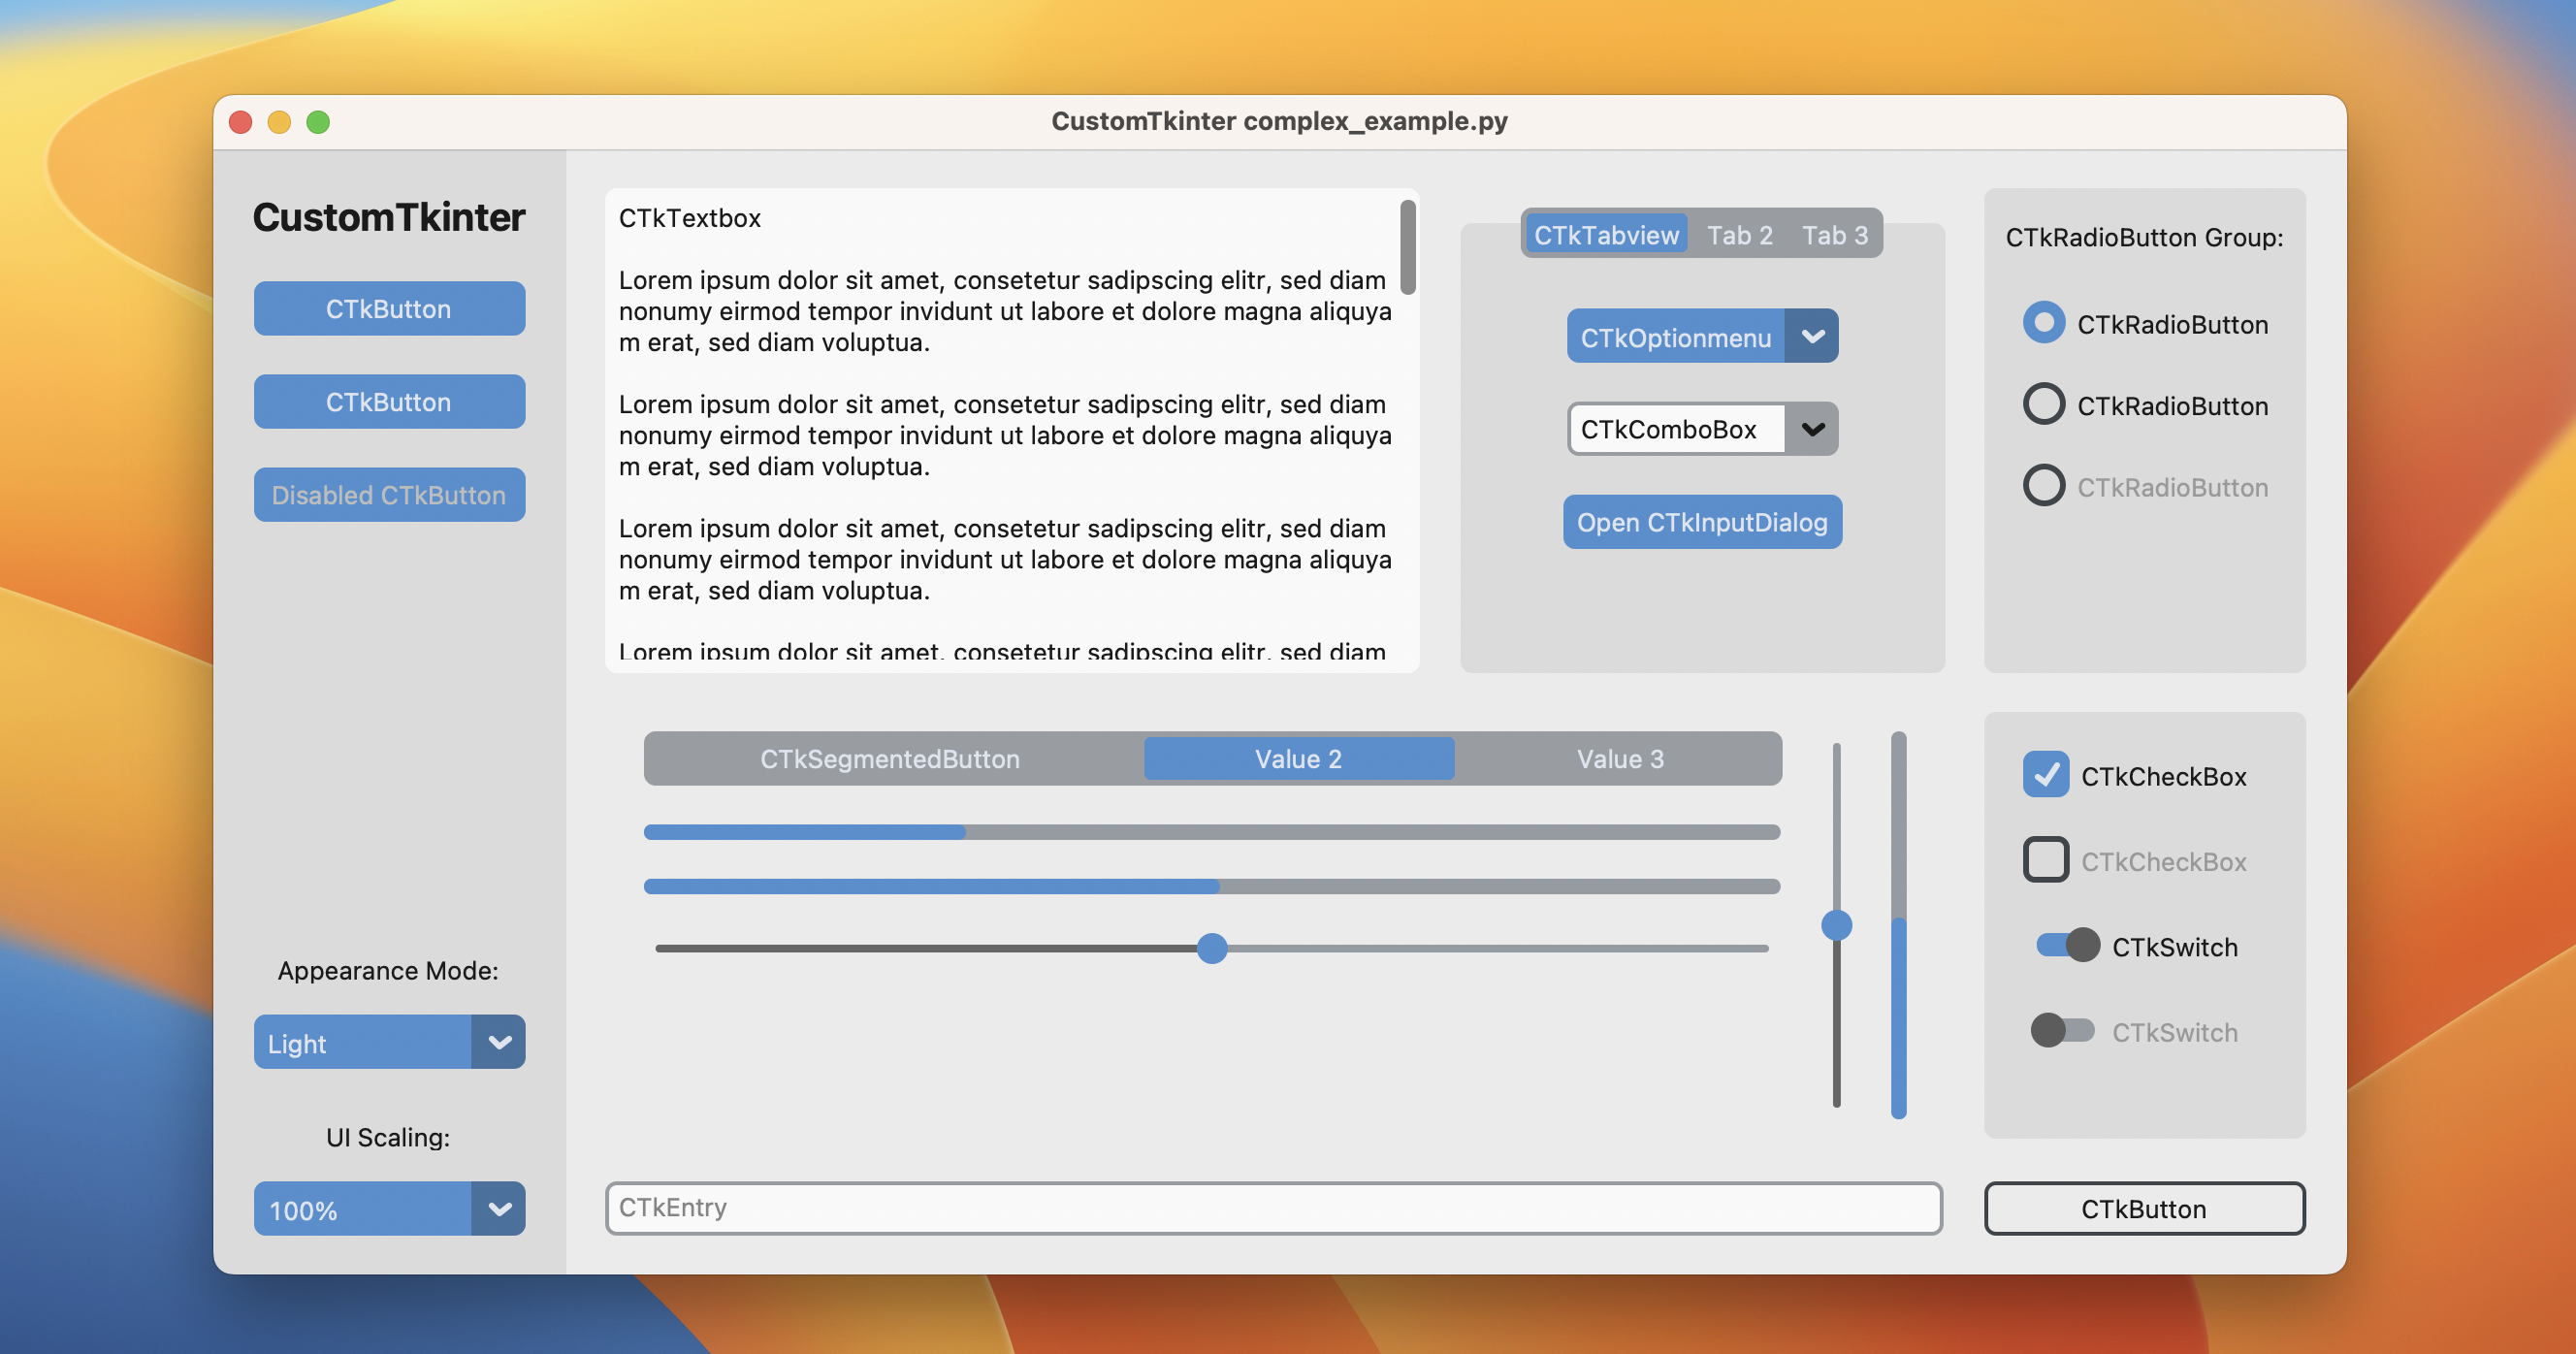
\includegraphics[width=0.90\textwidth]{ctk_example_light}
		\caption{Beispiel Modus \enquote{light} \label{fig:ctk_light}}
	\end{subfigure}
	\begin{subfigure}[t]{0.90\textwidth}
		\centering
		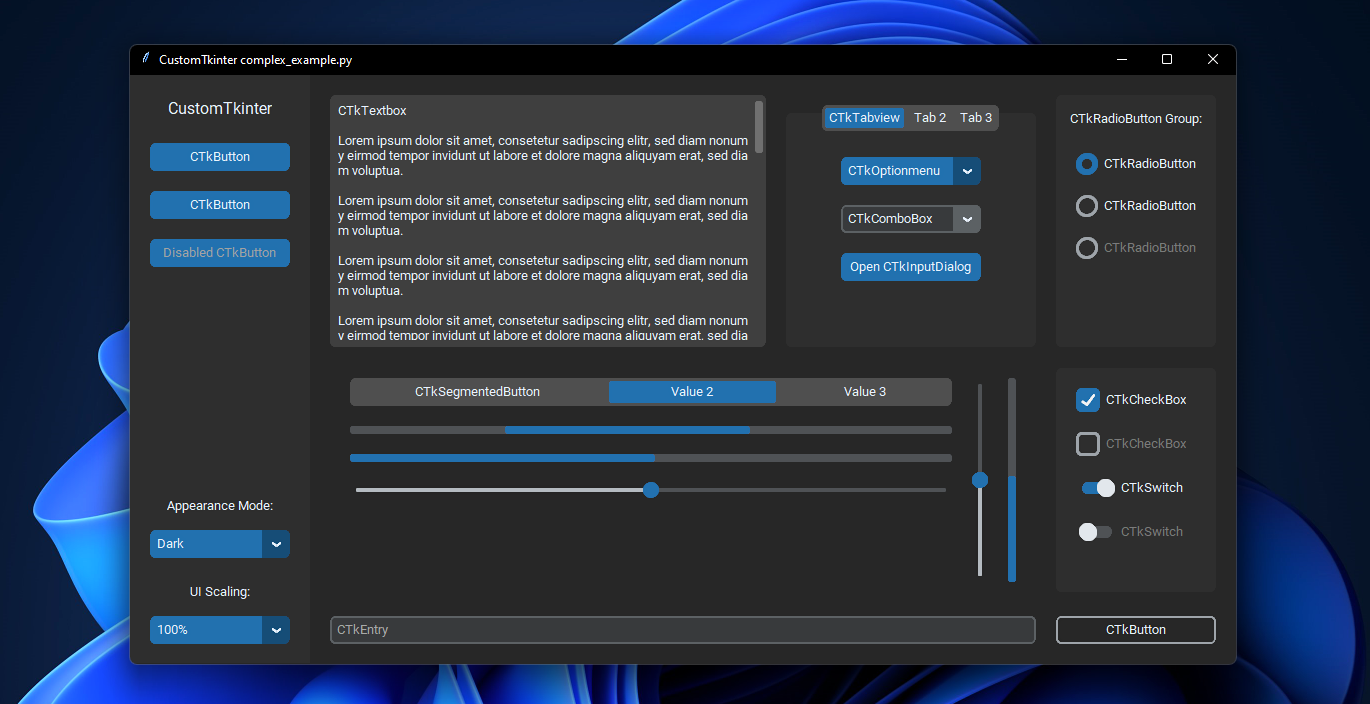
\includegraphics[width=0.90\textwidth]{ctk_example_dark}
		\caption{Beispiel Modus \enquote{dark} \label{fig:ctk_dark}}
	\end{subfigure}
	\caption{\gls{gls_ctk} Beispiele mit unterschiedlichen Modi und \enquote{blue} Theme  (Quelle: \url{https://github.com/tomschimansky/customtkinter?tab=readme-ov-file})    \label{fig:ctk_bsp}}
\end{figure}

Die regelmäßigen Updates für \gls{gls_ctk} sind ein weiterer Vorteil der Bibliothek. Darüber hinaus bietet die offizielle \gls{gls_ctk} Webseite eine übersichtliche und hilfreiche Dokumentation. In Kombination mit der zeitgemäßen Benutzeroberfläche übertrifft somit \gls{gls_ctk} das \enquote{tkinter.ttk} Untermodul von \gls{gls_tk}.


